\chapter{MÔ PHỎNG HOẠT ĐỘNG CỦA ROBOT}
     \section{Mô phỏng chuyển động của robot}
          \hspace*{0.6cm}Thực hiện mô phỏng chuyển động của Robot sau khi nhúng hàm truyền động cơ
          bộ điều khiển tốc độ động cơ, sai số cảm biến cùng với bộ điều khiển vị trí bám line  với các thông số như sau:
          \begin{table}[h]
               \centering
               \begin{tabular}{|l|c|}
               \hline
               \multicolumn{2}{|c|}{\textbf{Thông số hình học}} \\
               \hline
               Bán kính bánh xe, $r$ & 68 mm \\
               \hline
               Khoảng cách từ tâm dây cảm biến để trực dẫn dòng, $a$ & 50 mm \\
               \hline
               Khoảng cách đọc trục giữa 2 bánh xe, $b$ & 200 mm \\
               \hline
               \multicolumn{2}{|c|}{\textbf{Thời gian}} \\
               \hline
               Thời gian lấy mẫu bộ điều khiển động cơ, $\Delta t_1$ & 0.01 s \\
               \hline
               Thời gian lấy mẫu bộ điều khiển bám line, $\Delta t$ & 0.05 s \\
               \hline
               \multicolumn{2}{|c|}{\textbf{Bộ điều khiển PID}} \\
               \hline
               Hệ thống & $K_P = 0.078$; $K_D = 0.015$ \\
               \hline
               Động cơ 1 & $K_P = 1.0852$; $K_I = 13.6563$ \\
               \hline
               Động cơ 2 & $K_P = 1.0673$; $K_I = 13.948$ \\
               \hline
               \multicolumn{2}{|c|}{\textbf{Thông số động học}} \\
               \hline
               Vận tốc của robot, $v$ & 500 mm/s \\
               \hline
               Vận tốc của robot lúc vào cua, $v$ & 300 mm/s \\
               \hline
               Góc lệch ban đầu, $p$ & $\pi$ \\
               \hline
               \end{tabular}
               \label{tab:robot_specifications}
               \caption{Thông số đầu vào mô phỏng chuyển động của robot}
          \end{table}
     \section{Kết quả mô phỏng}
     \newpage
          \subsection{Khối hàng đỏ}
               \begin{figure}[H]
                    \centering
                    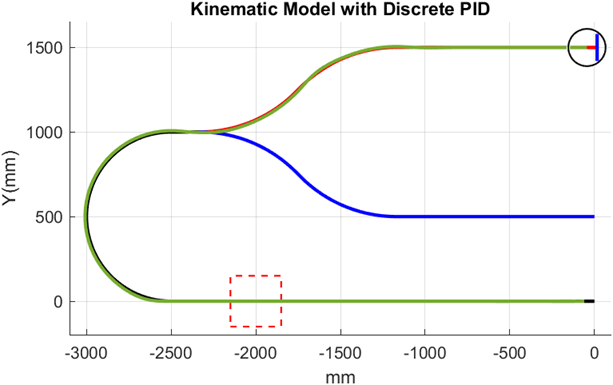
\includegraphics[width=1\textwidth]{pictures/chapter8/trajec_red.png}
                    \caption{Quỹ đạo đi khi nhận khối hàng đỏ}
                    \label{tra_red}
               \end{figure}
               \begin{figure}[H]
                    \centering
                    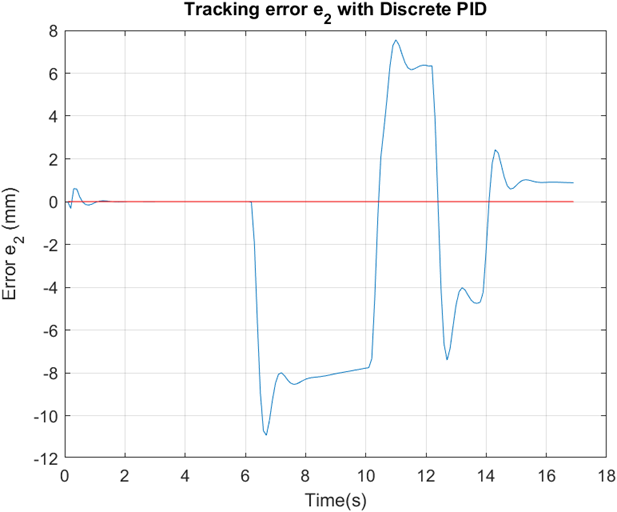
\includegraphics[width=0.8\textwidth]{pictures/chapter8/err_red.png}
                    \caption{Lỗi quỹ đạo e2 khi nhận khối hàng đỏ}
                    \label{err_red}
               \end{figure}
          \subsection{Khối hàng xanh}
               \begin{figure}[H]
                    \centering
                    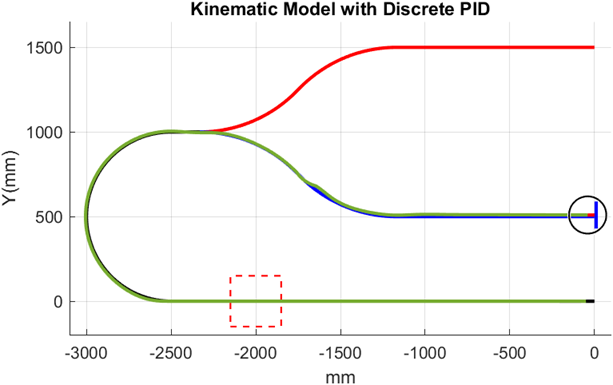
\includegraphics[width=0.8\textwidth]{pictures/chapter8/trajec_blue.png}
                    \caption{Quỹ đạo đi khi nhận khối hàng xanh}
                    \label{tra_blue}
               \end{figure}
               \begin{figure}[H]
                    \centering
                    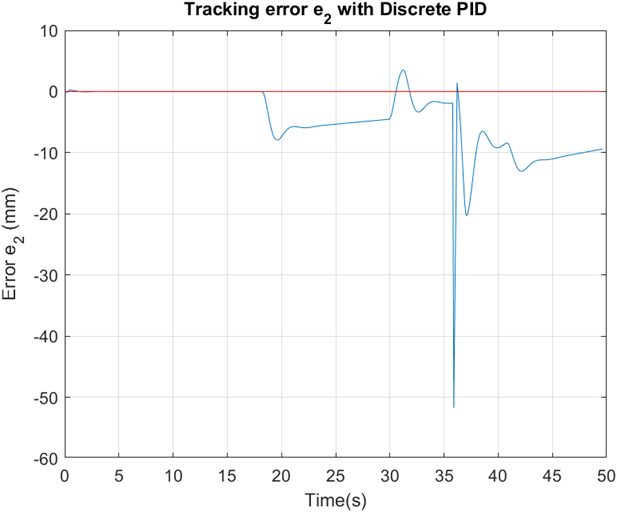
\includegraphics[width=0.8\textwidth]{pictures/chapter8/err_blue.png}
                    \caption{Lỗi quỹ đạo e2 khi nhận khối hàng xanh}
                    \label{err_blue}
               \end{figure}